Today there are several products either already on the market or under development that are more or less similar to Google Glass. Following is a short list describing some of the competition Google Glass faces.

\begin{itemize}
\item \textbf{Microsoft Hololens}\cite{hololens} 

Microsoft's offer in the augmented reality device space is a HUD that displays information over both of the user's eyes, called Microsoft Hololens, seen in Figure \ref{imagesSimilarProducts} (a). The intention, according to Microsoft, is not to be an immediate competitor to Google Glass. Microsoft's aim is not to make the same device as Google Glass. Google Glass is meant to be worn all the time, at all times. Microsoft Hololens is rather a device users only puts on when they intend to use it.

But the mot striking difference between Microsoft Hololens and Google Glass lies in the interaction with the real world. Google Glass is a two dimensional (2D) display that sits slightly above the users line of sight (see section \ref{subsec:googleglass}). Microsoft Hololens, on the other hand, is meant to interact with the world even further.

Microsoft intends to give the user tools to work in a three dimensional (3D) space. Microsoft's concept video\cite{hololensConceptVideo} of Microsoft Hololens shows examples of 3D modelling with the use of kinetic hand-movement detection, meaning that users will be able to see what they are working on from different angles simply by walking around it, just as if the object in question was real and had a physical mass.

\item \textbf{Recon Jet}\cite{reconJet}

Recon Jet, seen in Figure \ref{imagesSimilarProducts} (b) is a HMD developed by Recon Instruments. Recon Jet is suited for athletes. Because of the target audience Recon Jet has been fitted with a display that has high contrast in order to give good readability in high ambient lighting. The display's virtual image appears as  a 30 inch wide screen at approximately 2 meters distance,\cite{reconJetSpecs} to be compared with Google Glass' virtual image which, as stated in section \ref{subsec:googleglass},  appears as a 25 inch high definition screen seen from a distance of 2.5 meters.

Unlike Google Glass, Recon Jet's display is located below the user's line of sight, as seen in Figure \ref{imagesSimilarProducts}. Recon Jet's target audience, athletes, are used to having their information below line of sight. For instance a bike may have dashboard mounted to the handbar, or an athlete might be using a watch to check the time. Google wanted the Google Glass to be available to the user when the user wanted to use Google Glass, and to stay out of the way when the user did not want to use Google Glass. The location of the display and the brightness of the display indicates that the Recon Jet is meant to be used while the athlete is working out and not more regularly.

\item \textbf{GlassUp}\cite{glassUp}

GlassUp is an Italian company that received most of its founding for the HMD device, GlassUp (seen in Figure \ref{imagesSimilarProducts}), through the crowd-funding site Indiegogo.\cite{glassUpIndiegogo} GlassUp has been accused for being to similar to Google Glass, partially because of the name of the device.\cite{glassUpLegal} GlassUp does however make distinctions between the two products. On GlassUp's Indiegogo page the company made the comparison that looking at Google Glass' display was similar to looking in the back view mirror while GlassUp was similar to looking out the windscreen. The comparison referenced the fact that Google Glass' display is located above the user's line of sight, similar to a rear view mirror.

GlassUp instead displays information close to the center of the user's line of sight. GlassUp claimed, on the company's Indiegogo page, that the display was placed closer to the center of the users line of sight so that there would be less strain on the user's eyes. However, the biggest difference from Google Glass is that GlassUp is meant only to act as a second screen. GlassUp is a ``receive only'' device which displays information from the device currently connected through bluetooth, for instance a smartphone. GlassUp does not do any calculations on its own and must stay connected to a bluetooth device in order to display information.\cite{glassUpIndiegogo}

\item \textbf{C Wear Interactive Glasses}\cite{penny}

C Wear Interactive Glasses, seen in Figure \ref{imagesSimilarProducts}, is an industry focused device developed by Penny in V{\"a}ster{\aa}s, Sweden. C Wear Interactive Glasses projects an image onto the actual glass in front of the user's right eye and as such covers a larger area than similar devices such as Google Glass, Recon Jet and GlassUp. The projection is transparent which enables users to still see in front of them.\cite{pennyDisplay}

Being industry focused C Wear Interactive Glasses has also implemented a hands-free user interface  which does not require voice command. C Wear Interactive Glasses uses a jaw sensor which lies against the user's jawbone muscle. The sensor detects tension in the muscle, which registers as a click.\cite{pennyProducts}

C Wear Interactive Glasses, similar to GlassUp, is designed to be connected to an external device.\cite{pennyProducts} However, where GlassUp were to be connected through bluetooth C Wear Interactive Glasses is connected through an adapter which can send data and visual information via USB and HDMI. The external device can be a smartphone, a tablet, a PC or even a TV.
\end{itemize}
\hfill

	\begin{figure}[ht!]
		\centering
    	\subfloat[Microsoft Hololens\cite{hololens}]{{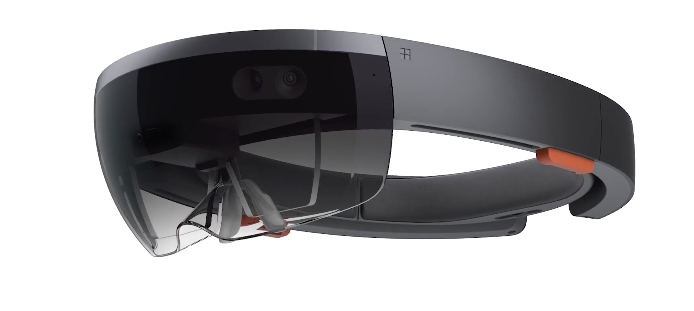
\includegraphics[width=65mm]{images/similarProducts/hololens}}}
    \qquad
    	\subfloat[Recon Jet\cite{reconJet}]{{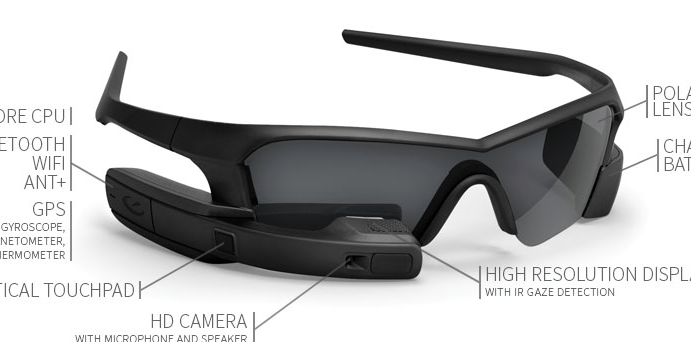
\includegraphics[width=65mm]{images/similarProducts/reconJet}}}
    \qquad
        \subfloat[GlassUp\cite{glassUpFeatures}]{{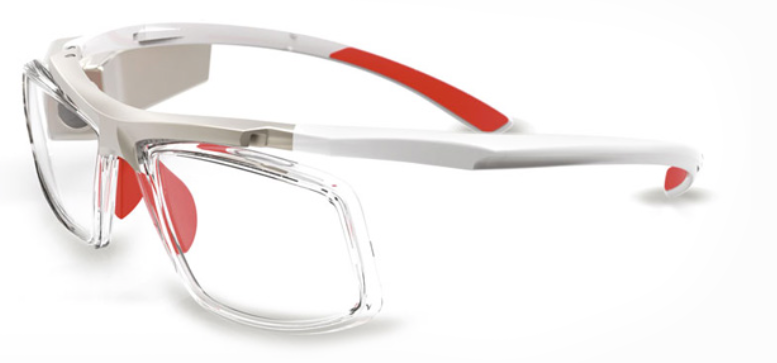
\includegraphics[width=65mm]{images/similarProducts/glassUp}}}
    \qquad
  	\subfloat[C Wear Interactive Glasses\cite{pennyProducts}]{{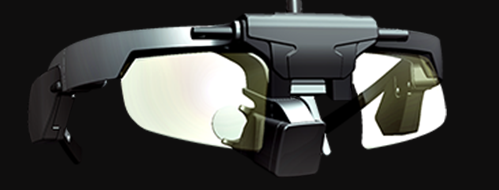
\includegraphics[width=65mm]{images/similarProducts/penny}}}
    \qquad
		\caption{Today there are many OHMD devices, either already on the market or under development. A more extensive list of devices can be found on wikipedia.\cite{ohmdWiki}}
		\label{imagesSimilarProducts}
	\end{figure}
	
%\url{http://www.microsoft.com/microsoft-hololens/en-us}
%\url{http://www.searchenginejournal.com/google-glass-alternatives/67018/}
%\url{http://www.penny.se}